\section{Dataset Description}

Fashion-MNIST was introduced by Xiao et al.\ as a drop-in replacement for MNIST \cite{xiao2017fashion}. It contains Zalando clothing images and is distributed through the \texttt{torchvision.datasets.FashionMNIST} interface. The project is released under the MIT license.

\begin{table}[H]
    \centering
    \caption{Dataset summary.}
    \label{tab:dataset-summary}
    \begin{tabularx}{\textwidth}{@{}lX@{}}
        \toprule
        Property & Description \\
        \midrule
        Source and interface & Fashion-MNIST through torchvision 0.29.0. \\
        Collection and labeling & Centered $28\times28$ grayscale product images with one integer class label per image. \\
        Number of samples & 60,000 official training images and 10,000 official test images. \\
        Classes & T-shirt/top, Trouser, Pullover, Dress, Coat, Sandal, Shirt, Sneaker, Bag, and Ankle boot. \\
        Storage and formats & IDX image/label files plus gzip archives under \texttt{Assignment1/data/FashionMNIST/raw}; approximately 82 MB including compressed and extracted copies. \\
        Biases and limitations & Small centered grayscale objects, limited background variation, low resolution, and substantial visual overlap among upper-body garments. \\
        \bottomrule
    \end{tabularx}
\end{table}

\begin{figure}[H]
    \centering
    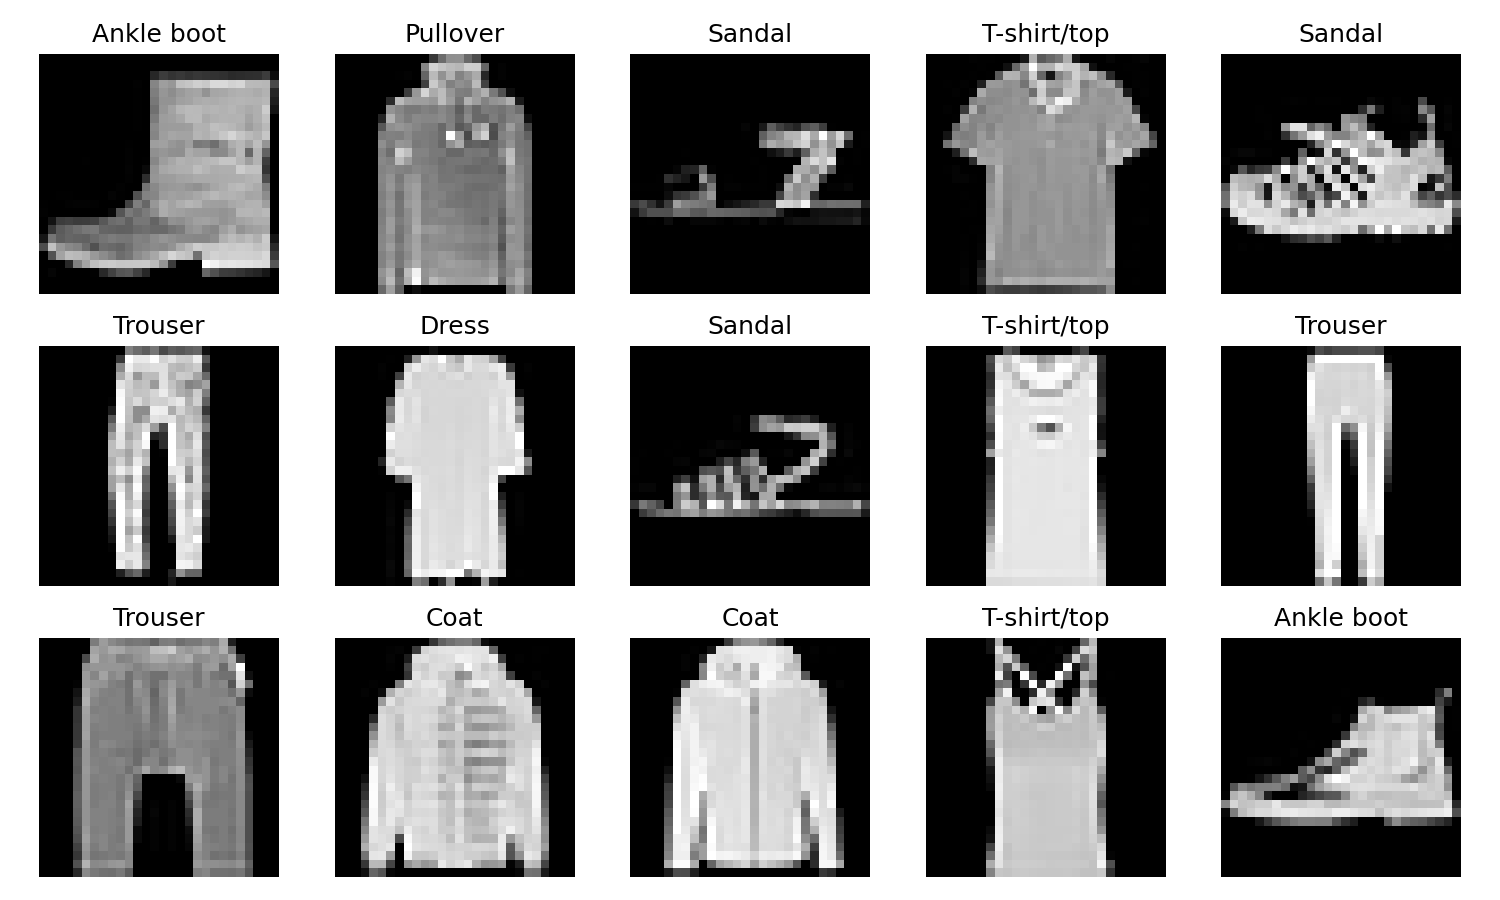
\includegraphics[width=0.9\textwidth]{../../Assignment1/outputs/eda/random_examples.png}
    \caption{Representative Fashion-MNIST examples selected reproducibly with seed 42.}
    \label{fig:preprocessed-batch}
\end{figure}

\begin{table}[H]
    \centering
    \caption{Official training-pool class distribution.}
    \label{tab:target-distribution}
    \begin{tabular}{@{}lrr@{}}
        \toprule
        Class / target & Count & Percentage \\
        \midrule
        T-shirt/top & 6,000 & 10\% \\
        Trouser & 6,000 & 10\% \\
        Pullover & 6,000 & 10\% \\
        Dress & 6,000 & 10\% \\
        Coat & 6,000 & 10\% \\
        Sandal & 6,000 & 10\% \\
        Shirt & 6,000 & 10\% \\
        Sneaker & 6,000 & 10\% \\
        Bag & 6,000 & 10\% \\
        Ankle boot & 6,000 & 10\% \\
        \midrule
        Total & 60,000 & 100\% \\
        \bottomrule
    \end{tabular}
\end{table}

The classes are perfectly balanced in the official training pool. Stratified splitting therefore preserves 5,400 training and 600 validation examples per class, so accuracy is meaningful and macro-F1 remains useful for exposing class-specific weaknesses rather than correcting a frequency imbalance.
